\section{Syntax-Directed Definitions}
A Syntax-Directed Definition (SDD) is a context-free grammar in which:
\begin{itemize}
	\item each symbol can have an associated set of attributes (numbers, types, table references, strings, memory locations, \ldots);
	\item each production can have an associated set of semantic rules (evaluating attributes, interacting with the symbol table, writing lines of intermediate code to a buffer, printing messages, \ldots).
\end{itemize}

\subsection{Inherited and Synthesized Attributes}
A semantic rule associated with a production $A \to XYZ$ can refer only attributes associated with symbols in that production:
\begin{description}
	\item[Inherited Attributes] are evaluated in rules where the associated symbol is on the right side of the production;
	\item[Synthesized Attributes] are evaluated in rules where the associated symbol is on the left side of the production.
\end{description}

\begin{table}[h]
	\centering
	\begin{tabular}{l|l}
		Productions & Semantic Rules \\ \hline
		$L \to Em$ & $print(E.val)$ \\ \hline
		$E \to E_1 + T$ & $E.val = E_1.val + T.val$ \\ \hline
		$E \to T$ & $E.val = T.val$ \\ \hline
		$T \to T_1 \ast F$ & $T.val = T1_.val \ast F.val$ \\ \hline
		$F \to digit$ & $F.val = digit.lexval$
	\end{tabular}
	\caption{SDD example for a desk calculator.}
\end{table}
Each of the non-terminal $E, T, F$ has a single synthesized attribute, named ``val''; the terminal digit has an attribute ``lexval'' which is the integer value returned by the scanner.

\begin{table}[h]
	\centering
	\begin{tabular}{l|l}
		Productions & Semantic Rules \\ \hline
		$D \to TL$ & $L.inh = T.type$ \\ \hline
		$T \to int$ & $T.type = integer$ \\ \hline
		$T \to float$ & $T.type = real$ \\ \hline
		$L \to L_1, id$ & $L_1.inh = L.inh; addtype(L.inh, id.entry)$ \\ \hline
		$L \to id$ & $addtype(L.inh, id.entry)$
	\end{tabular}
	\caption{SDD example for simple declarations.}
\end{table}

\begin{itemize}
	\item the non-terminal $T$ has a synthesized attribute named $type$;
	\item the non-terminal $L$ has a inherited attribute, named $int$;
	\item the terminal $id$ has an attribute entry which is the value returned by the scanner (it points to the symbol table entry for the identifier associated with $id$);
	\item the function $addtype(L.inh, id.entry)$ installs the type $L.inh$ at the symbol table position $id.entry$.
\end{itemize}

\subsection{Evaluation Orders for Syntax Directed Definitions}
An attributes at a node in an annotated parse tree cannot be evaluated before the evaluation of all attributes upon which its value depends.
The dependency relations in a parse tree define a dependency graph representing the flow of information among attributes and semantic rules.
Any topological sort of the dependency graph is an allowable order of evaluation for an SDD.
Any directed acyclic graph has at least one topological sort.

\subsection{Ordering the Evaluation of SDD}
Syntax-directed translation can be performed by:
\begin{itemize}
	\item creating a parse tree;
	\item visiting the parse tree an evaluating an SDD according to a topological sort of the dependency graph.
\end{itemize}
It is extremely complex to tell whether, for a given SDD, there are any parse trees whose dependency graphs have cycles.
It is possible to define classes of DSS (S-attribtues and L-attributes) in ways that:
\begin{itemize}
	\item cycles are not allowed;
	\item translation is performed in connection with top-down or bottom-up parsing, without explicitly creating the tree nodes.
\end{itemize}

\subsection{S-Attributes Definitions}
An SDD is S-attributed if every attribute is synthesized.
All semantic rules use only attributes of symbols in the right side of the associated productions.

\begin{table}[h]
	\centering
	\begin{tabular}{l|l}
		Productions & Semantic Rules \\ \hline
		$L \to En$ & $print(E.val)$ \\ \hline
		$E \to E_1 + T$ & $E.val = E_1.val + T.val$ \\ \hline
		$E \to T$ & $E.val = T.val$ \\ \hline
		$T \to T_1 \ast F$ & $T.val = T_1.val \ast F.val$ \\ \hline
		$T \to F$ & $T.val = F.val$ \\ \hline
		$F \to (E)$ & $F.val = E.val$ \\ \hline
		$F \to digit$ & $F.val = digit.lexval$ 
	\end{tabular}
\end{table}

\begin{figure}[H]
	\centerline{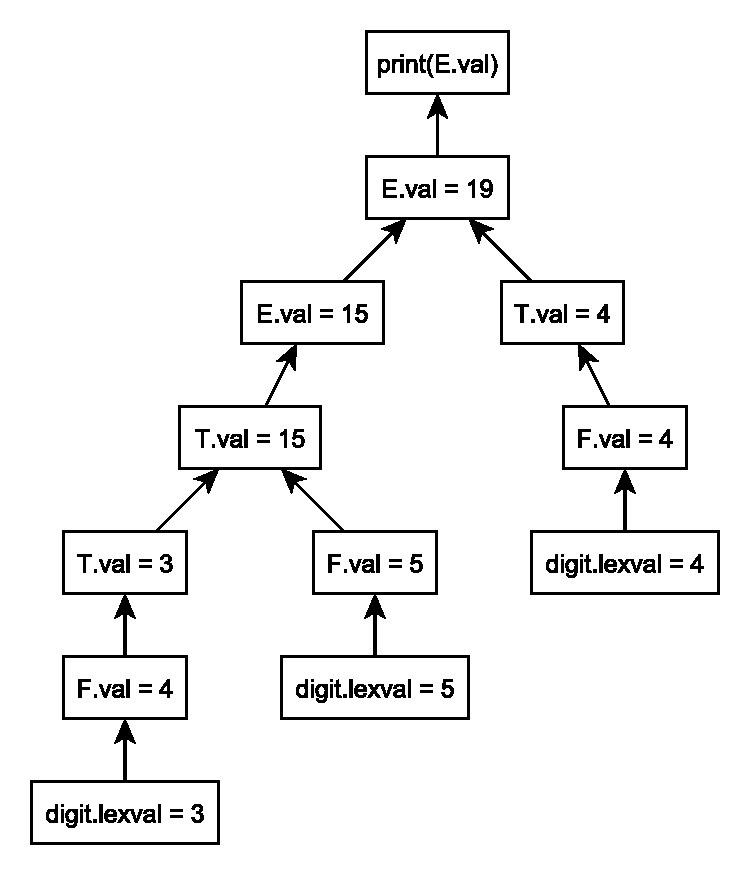
\includegraphics[width=0.6\textwidth]{img/14.pdf}}
	\caption{Dependency trees of S-attributed definitions}
\end{figure}

\subsection{Evaluation Order for S-Attributed Definitions}
S-Attributed definitions can be evaluated in any bottom-up order.
The evaluation order of function post-order (rootNode) corresponds to the order in which a bottom-up parser creates nodes in a parse tree.

\section{Syntax-Directed Translation Schemes (SDT)}
